\documentclass[journal]{IEEEtran}
% IEEE Transactions on Industrial Informatics -- anonymous regular-paper draft
% Compile: latexmk -pdf main.tex
\usepackage{amsmath,amssymb,amsfonts}
\usepackage{algpseudocode}
% Local XeTeX/Tectonic builds: route IEEEtran's ptm (Times) family requests to
% the legacy Times Type1 faces so metrics match the pdfLaTeX reference build;
% the latexmk -pdf (pdfLaTeX) path is unaffected.
\usepackage{iftex}
\ifxetex
  \DeclareFontFamily{TU}{ptm}{}
  \DeclareFontShape{TU}{ptm}{m}{n}{<->ptmr8t}{}
  \DeclareFontShape{TU}{ptm}{b}{n}{<->ptmb8t}{}
  \DeclareFontShape{TU}{ptm}{m}{it}{<->ptmri8t}{}
  \DeclareFontShape{TU}{ptm}{b}{it}{<->ptmbi8t}{}
  \DeclareFontShape{TU}{ptm}{m}{sl}{<->ptmro8t}{}
  \DeclareFontShape{TU}{ptm}{m}{sc}{<->ptmr8t}{}
\fi
\usepackage{graphicx}
\usepackage{booktabs}
\usepackage{tabularx}
\usepackage{array}
\usepackage[table]{xcolor}
\usepackage{stfloats}
\usepackage{placeins}
\usepackage{url}
\usepackage{etoolbox}
\urlstyle{same}
% Cross-references and citations. The cite package renders IEEE-style citation
% groups ([14]--[16], [20], [21]) with hyperref support.
\usepackage{cite}
\usepackage[colorlinks=true,linkcolor=black,citecolor=black,urlcolor=black]{hyperref}
\hypersetup{bookmarksnumbered=true,
  pdftitle={Governed Setpoint Writing for Industrial Agents: A Configuration-Driven Runtime and Simulated Evaluation},
  pdfauthor={},
  pdfsubject={IEEE Transactions on Industrial Informatics},
  pdfkeywords={industrial agents, governed setpoint writing, industrial communication, simulation-based evaluation, system integration}}

% Float placement only; IEEEtran margins and body type remain unchanged.
\setcounter{topnumber}{4}
\setcounter{bottomnumber}{3}
\setcounter{totalnumber}{7}
\setcounter{dbltopnumber}{1}
\renewcommand{\topfraction}{0.95}
\renewcommand{\bottomfraction}{0.80}
\renewcommand{\textfraction}{0.03}
\renewcommand{\floatpagefraction}{0.72}
\renewcommand{\dbltopfraction}{0.95}
\renewcommand{\dblfloatpagefraction}{0.72}

% Tight but conventional float separation; body type and margins are unchanged.
\setlength{\textfloatsep}{8pt plus 2pt minus 3pt}
\setlength{\dbltextfloatsep}{8pt plus 2pt minus 3pt}
\setlength{\intextsep}{7pt plus 2pt minus 3pt}
\setlength{\abovecaptionskip}{3pt plus 1pt minus 1pt}
\setlength{\belowcaptionskip}{2pt plus 1pt minus 1pt}

\newcommand{\system}{the platform}
% Acknowledgment is omitted from this blinded review copy. See the separate
% submission-only disclosure draft and confirm its destination with TII.

\begin{document}
\bstctlcite{IEEEbstctl}

\title{Governed Setpoint Writing for Industrial Agents: A Configuration-Driven Runtime and Simulated Evaluation}

\author{}
\markboth{IEEE Transactions on Industrial Informatics, Submitted Manuscript}{Governed Setpoint Writing}

\maketitle

\begin{abstract}
Industrial agents can propose process changes, but a runtime must resolve each proposal against active production context, identify the intended control point, and enforce route-specific limits before dispatch. We present a configuration-driven runtime that binds production context and directional signal mappings to shared dispatch. Operation handlers perform route-specific authorization and revalidation, and a common write controller applies value guards. The runtime records command outcomes, optional device readbacks, and later process observations separately.
Across four simulated scenes, 220/220 admissible mapping requests were accepted, 219/219 collected structural-range requests were rejected, and 216/216 available simulator readbacks matched. A mock-driver ablation returned HTTP 400 for six process-window violations with the interlock enabled and HTTP 200 when it was removed. In a preregistered exploratory fixed-horizon comparison of the scripted recipe policy with no-write, 9 of 11 attempts yielded valid pairs; all nine had lower IAE under the script, with per-scene median reductions of 165.2~g\,s, 615.6~mg/L\,s, and 8000.5~HV\,s. Two pairs were invalid because of sampling gaps. A separate three-episode LLM-driven simulator pilot ended canceled and below target in every episode; the local recorder reported two writes per episode. These results are limited to the tested simulator and mock-driver paths. They do not establish general control efficacy, autonomous task success, or physical-plant safety.
\end{abstract}

\begin{IEEEkeywords}
Industrial agents, governed setpoint writing, industrial communication,
simulation-based evaluation, system integration.
\end{IEEEkeywords}

\IEEEpeerreviewmaketitle

\section{Introduction}
\IEEEPARstart{I}{ndustrial} agents can propose process changes, but a runtime must resolve the production context and map each proposal to the intended control signal before dispatch. That mapping depends on the scene. On a cast-film line, for example, a line-speed setpoint may affect film thickness, yet the setpoint and thickness measurement remain distinct variables even when both use Message Queuing Telemetry Transport (MQTT). A service receipt, a device readback, and a later process measurement also record different events. Fig.~\ref{fig:control-path} illustrates these distinctions.

Prior work addresses industrial-agent planning and control, programmable logic controller (PLC) program generation, protocol access, semantic commissioning, and plant-facing verification. Because these studies use different tasks and evaluation settings, their results are not directly comparable. This paper examines a narrower question: how should a runtime carry production context and signal meaning from a task-level proposal to device dispatch, while checking route-specific authority and limits? We do not propose a new planning policy or control law.

We implement this path in a configuration-driven runtime. Each scene binds its line, product, recipe, and run to separate acquisition and control nodes, registered drivers, process objectives, and write limits. Task-mediated and direct calls share a dispatcher, after which the selected handler resolves current state and applies its route-specific checks. Approval paths then revalidate the state relevant to that operation: recipe operations check the active context, while single-node writes check their binding and any applicable grant before the common controller checks the value. These checks reduce exposure to stale state, but they do not make authorization and device I/O atomic.

The contributions are:
\begin{enumerate}
  \item A production-scene configuration model that links operational context and direction-specific signal mappings to registered drivers, objectives, and limits at the operation boundary (Section~III).
  \item An implemented task-to-device path for registered agent harnesses and direct callers. It combines shared dispatch, route-specific checks, conditional approval, and common write guards, while retaining command outcomes, optional readbacks, and later process observations as separate records (Sections~III--V).
  \item An evidence-bounded evaluation of configured mappings and pre-dispatch guards across four simulated scenes, with command readback, process observations, and live-Agent outcomes reported separately (Section~VI).
\end{enumerate}

Section~II reviews industrial-agent, interface, and operation-governance work. Sections~III--V describe the runtime configuration, operation path, and write controls. Section~VI reports the evaluation by evidence type, and Section~VII discusses the limits of the results.

\begin{figure}[!b]
\centering
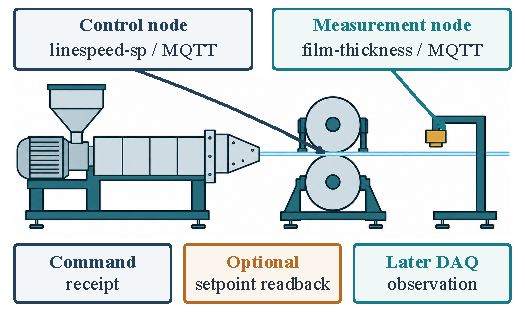
\includegraphics[width=0.98\columnwidth]{../figures/fig1.pdf}
\caption{Running cast-film example. MQTT maps the line-speed setpoint to a control node and film thickness to a separate measurement node. A command receipt, optional device readback, and later DAQ observation are distinct evidence; the illustration does not establish a causal process effect.}
\label{fig:control-path}
\end{figure}

\section{Related Work}
\label{sec:related}
Table~\ref{tab:related-comparison} summarizes the representative systems discussed below. Because they address different tasks, interfaces, and evaluation units, the comparison is qualitative rather than a ranking or head-to-head benchmark. A more detailed source list is provided in Table~S7-I.

\begin{table*}[!t]
\centering
\caption{Representative related work and the scope of its reported evaluation. The studies address different tasks and are not a common benchmark.}
\label{tab:related-comparison}
\footnotesize
\setlength{\tabcolsep}{5pt}
\begin{tabularx}{\textwidth}{@{}>{\raggedright\arraybackslash}p{0.16\textwidth}>{\raggedright\arraybackslash}p{0.40\textwidth}X@{}}
\toprule
Study & Main focus & Reported setting \\
\midrule
Biskupovic et al.~\cite{biskupovic2025supervision} & Agent-based industrial service selection and reselection & Service adaptability and performance in an industrial cyber--physical system \\
K\"{o}hle et al.~\cite{koehle2026llmdriven} & Module-specific agents and skill-based manufacturing & Nine simulated production challenges \\
Graul et al.~\cite{graul2026aas} & Grounded proposals, documented authorization, and PLC validation & Two laboratory proof-of-concept settings \\
Schall~\cite{schall2026safe} & Process-diagram, supervisory control and data acquisition (SCADA), and procedure-grounded verification & Five simulated scenarios and proposal evaluation \\
Vyas et al.~\cite{vyas2026detection} & Multi-agent fault-recovery planning with a process-plant twin & Mixing and stirred-tank reactor studies \\
This work & Scene-bound signal mappings, shared dispatch, and route-specific governance & Simulator and mock-driver probes, scripted missions, and exploratory live-Agent episodes \\
\bottomrule
\end{tabularx}
\end{table*}

\subsection{Industrial Agents and Plant Integration}
Research on industrial agents covers service selection, control generation, PLC programming, and production tasks. Biskupovic et al. study online service selection and reselection in industrial cyber--physical systems. Xia et al. present a digital-twin-connected automation architecture; related work generates PLC programs or incorporates human instructions into model-predictive control \cite{biskupovic2025supervision,xia2025architecture,xia2025control,liu2026agents4plc,wu2025instructmpc}. Li et al. use structured instructions, retrieval, and iterative verification to generate and check finite-element scripts for Abaqus, evaluating engineering-artifact generation rather than runtime authority over process writes \cite{li2026modsolagent}. Other studies examine language-model agents, manufacturing skills, and natural-language machine interaction \cite{koehle2026llmdriven,lim2025llmenabled,zhao2026shopfloor,hofmann2025nlc,huang2026made}. Vyas et al. pair multi-agent fault-recovery planning with plant-knowledge retrieval and Digital Process Plant Twin studies of mixing and continuous stirred-tank reactors (CSTRs) \cite{vyas2026detection}.

This work is complementary: it focuses on what happens after an agent proposes an operation. The runtime carries scene context and signal mappings to the selected route, then applies that route's checks before dispatch.

\subsection{Industrial Interfaces and Semantic Commissioning}
Agent-facing interface work includes Model Context Protocol (MCP) adapters for industrial protocols, semantic recipes built from Open Platform Communications Unified Architecture (OPC UA) skills, and tools that bind manufacturing data to a cognitive digital twin \cite{silva2025mcpmanufacturing,koehle2025semanticrecipes,xavier2026industriConnect,liu2026semanticcommissioning}. These systems address capability discovery, protocol access, or commissioning. In this runtime, configuration binds registered drivers to scene-specific read and write nodes; named operations resolve those bindings and pass through the checks for authority and write limits. MCP and a semantic node name are not authorization mechanisms.

\subsection{Governed Operations and Verification}
Prior work includes plant-facing verification. Graul et al. ground proposals in the Asset Administration Shell and combine documented human authorization with PLC-validated OPC UA Methods \cite{graul2026aas}. Schall checks proposals against piping and instrumentation diagrams, SCADA data, and standard operating procedures; Lin and Chen describe a policy-governed sensor--manufacturing execution system (MES)--enterprise resource planning (ERP) digital thread \cite{schall2026safe,lin2026agentic}. PLCBench evaluates autonomous agents against commercial PLCs using hardware-in-the-loop process simulation \cite{zhou2026plcbench}. The present implementation asks how configured signal bindings, route-specific checks, shared dispatch, and separate command and process records work together at the write boundary. This is a system-integration contribution; the studies use different settings and do not establish comparative safety.

\subsection{Production Context and Outcome Evidence}
MCP standardizes tool discovery and invocation, while the application remains responsible for operation-specific authority and process constraints \cite{mcp2024}. ISA-88 and ISA-95 define recipe and production-operation concepts \cite{isa88_2010,isa95_2025}. Run-to-run control connects process observations to subsequent decisions; human--automation research examines how responsibility is allocated between people and automation \cite{moyne2000r2r,parasuraman2000model}. These ideas inform the runtime's production context and evidence model. The implementation does not claim conformance to a complete ISA-88/95 information model, and its scripted approval fixture is not a human-factors evaluation.

\section{System Design}
\label{sec:design}
The runtime exposes named services through two entry paths: task-mediated calls through the collaboration runtime and a registered agent harness, and direct calls through the Representational State Transfer (REST) application programming interface (API) or the Model Context Protocol (MCP) over standard input/output (stdio). Both reach the shared dispatcher, as summarized in Fig.~\ref{fig:arch}.

\begin{figure*}[!t]
\centering
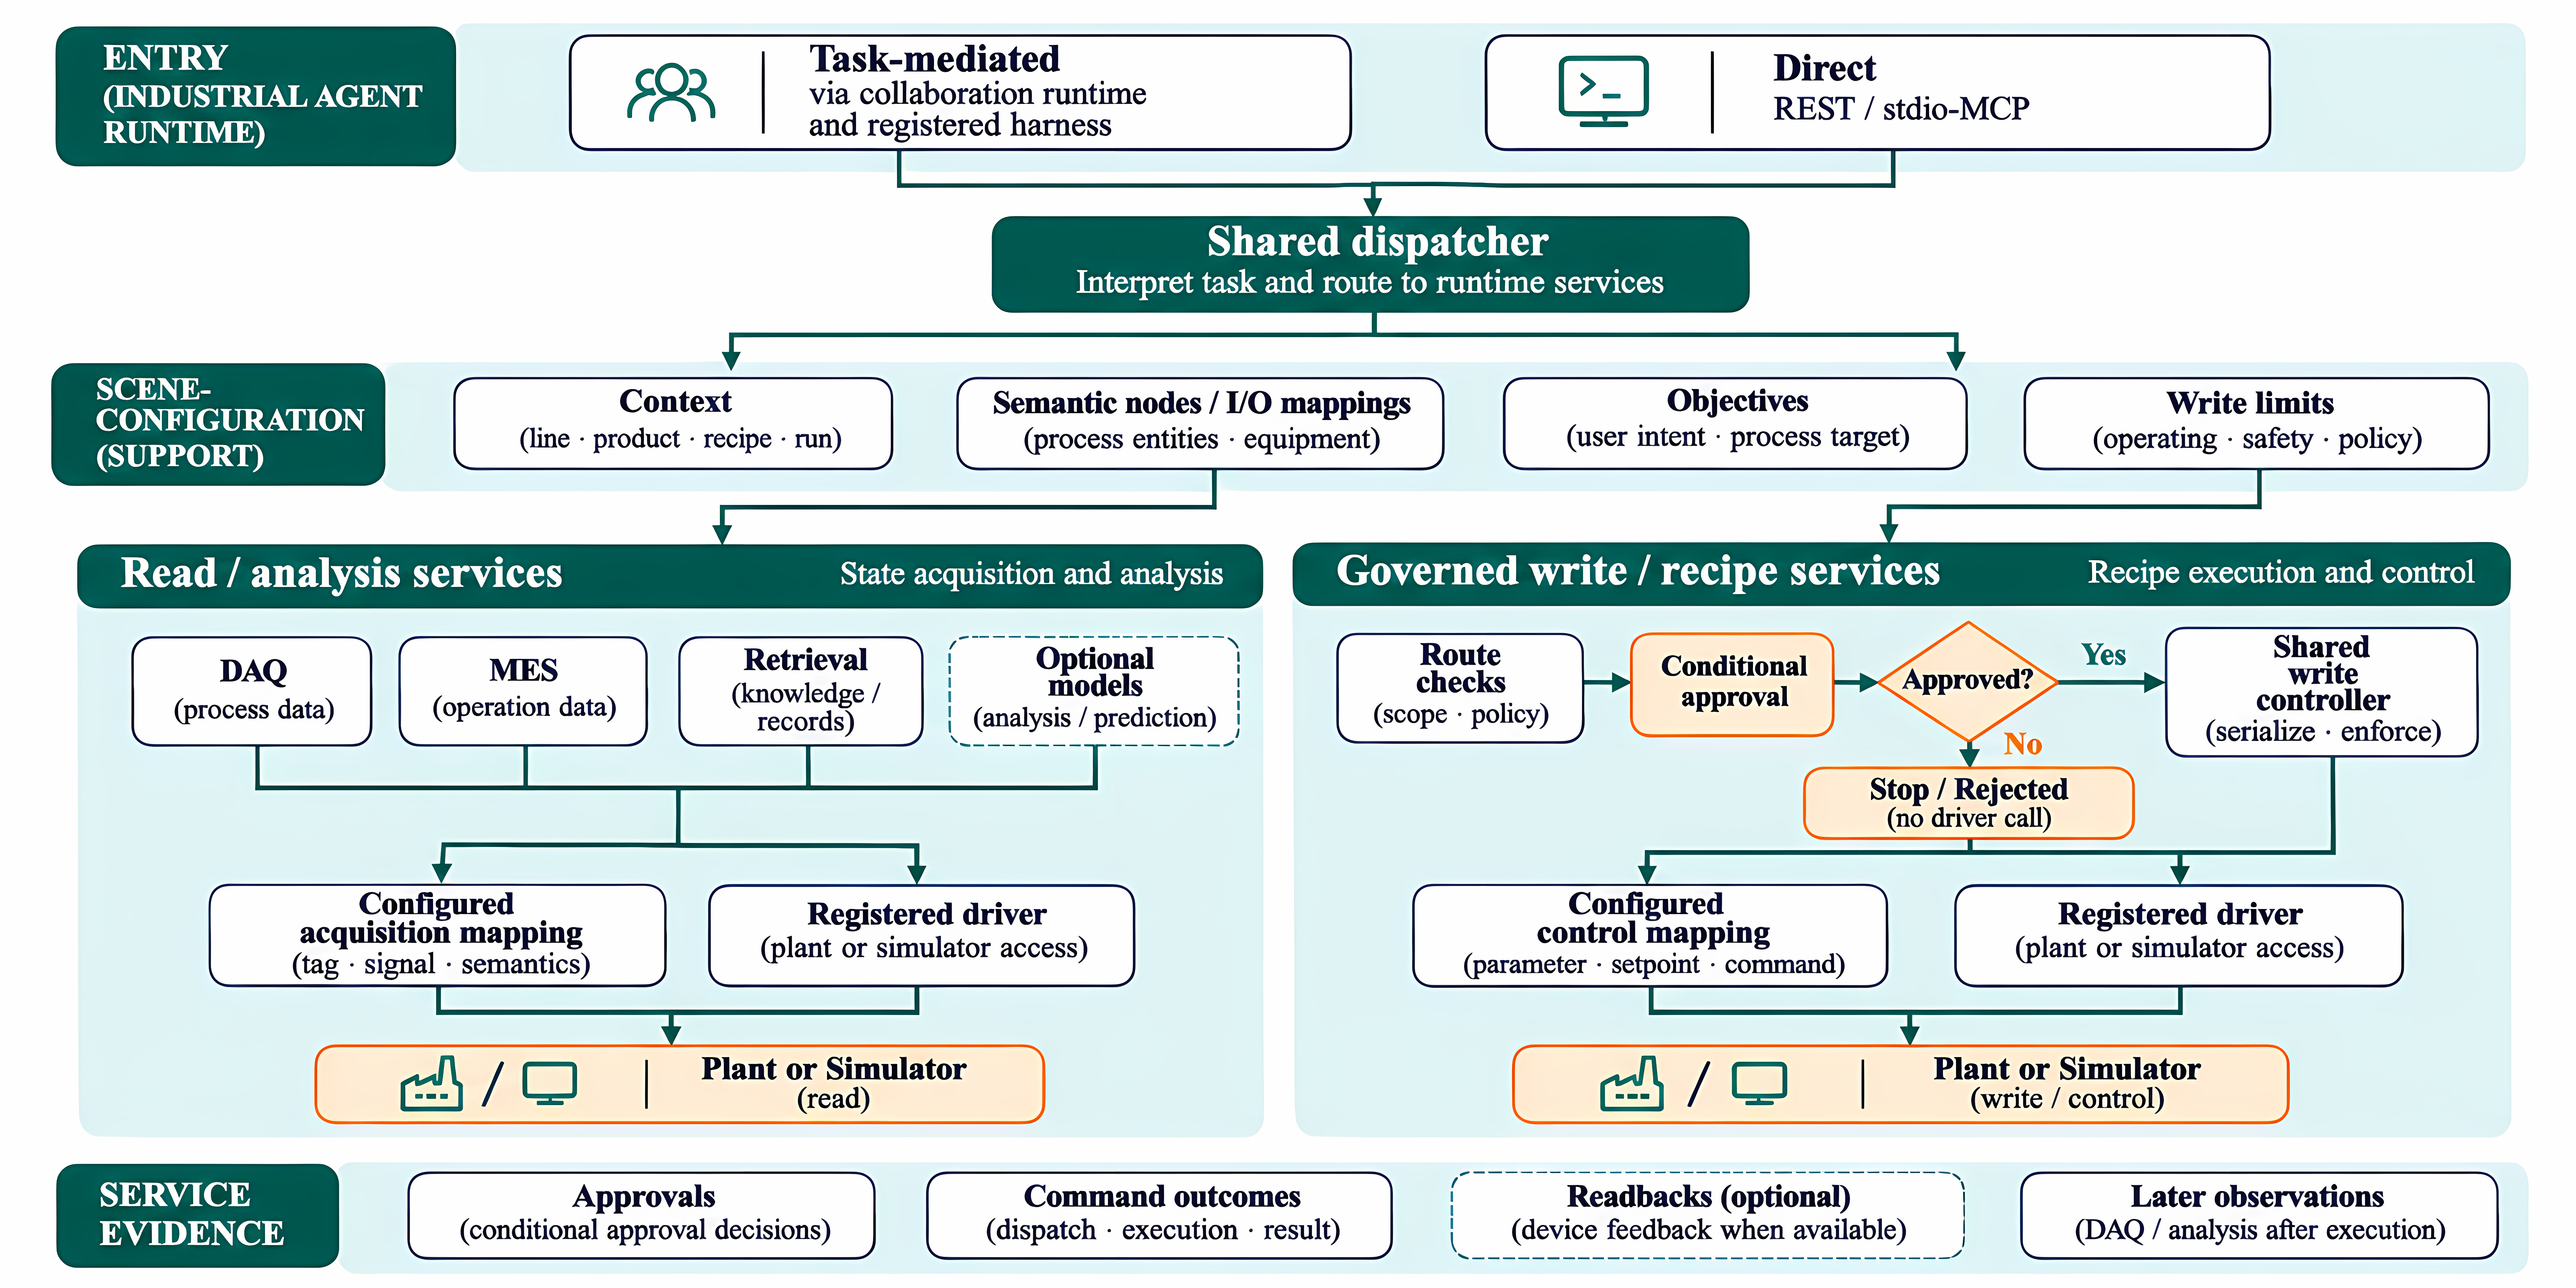
\includegraphics[width=\textwidth]{../figures/fig2.png}
\caption{Task-mediated and direct calls converge on the shared dispatcher, which routes requests to read/analysis or governed write/recipe services. The scene-configuration band supplies context, semantic I/O mappings, objectives, and write limits; it is configuration support rather than a third entry route. Read/analysis services connect DAQ, MES, retrieval, and optional models to acquisition mappings and registered drivers. The governed write path applies route checks and conditional approval before the shared write controller, then uses configured control mappings and drivers. The service-evidence band separates approvals, command outcomes, optional readbacks, and later observations. Evaluation uses simulator and mock-driver fixtures. The depicted limits are application checks and do not establish functional safety.}
\label{fig:arch}
\end{figure*}

\subsection{Design Rationale and Requirements}
\label{sec:principles}
The runtime must preserve process meaning across heterogeneous drivers,
provide a stable operation contract to registered harness adapters, and check
current authority and process limits before a write. It must also keep command
acceptance separate from later process observations. Scene configuration,
registered adapters, shared dispatch, route handlers, and service-owned
records implement these boundaries.

At task start, the context builder assembles the active production tuple and
relevant process summaries. This context informs a proposal but does not grant
write authority. When an operation is invoked, its handler resolves the live
state required by that route.

\subsection{Layered Architecture}
\label{sec:layers}
Task-mediated calls pass through the collaboration runtime, which coordinates
the task and invokes a registered harness adapter. The adapter presents the
agent's scoped tools and current task context; its binding and channel policy
constrain the available operations. Direct REST calls and the stdio-MCP
operation bridge skip task execution but converge on the same dispatcher. This
description applies to the operation bridge: MCP management and task methods
remain on their service routes.

Scene configuration has two consumers. The task route receives active context
and objectives, while operation services resolve node mappings and guards when
an operation executes. Read and analysis services group DAQ, MES data access,
retrieval, and optional models; write and recipe services handle control
operations. For a write mapping, the driver registry can select a configured
MES-REST adapter. At the field layer, input/output (I/O) mappings connect
semantic nodes to built-in or plugin drivers for a plant or simulator. Each
owning service retains its task, command, observation, or configuration
records and associates them with the actor and production context where
supported.

\subsection{Scene Configuration as the Integration Boundary}
\label{sec:scene-config}
Scene-specific process semantics are configured before an
agent task begins. The active line identifies the production context; product
and recipe records supply applicable targets and limits; the run record
provides the current operating state. Semantic nodes bind process variables
to direction-specific acquisition or control mappings, which the driver
registry resolves to supported protocol implementations. Here
\emph{semantic} denotes a named process variable with a direction, unit, and
configured mapping; it is not an OPC UA or Asset Administration Shell
information model. Each agent-facing operation is named and typed, so a harness does not need to
construct protocol-specific messages. A scene using an already registered
driver can supply different context and node mappings behind the same
operation contract. A protocol not present in the registry still requires a
driver adapter; configuration alone does not implement a new protocol.

In the cast-film simulator preset, for example, the MQTT command mapping
\texttt{linespeed-sp} controls line speed in m/min, while the distinct
\texttt{film-thickness} mapping supplies thickness in $\mu$m. A task can
refer to both nodes: a candidate is admitted against the control node's
limits, whereas a later DAQ observation describes thickness. Sharing MQTT does
not make either signal a substitute for the other.

Table~\ref{tab:scene-config} summarizes how the execution path uses the scene
description and distinguishes configuration-time bindings from checks against
live state. The context assembled for an agent turn is descriptive. Before a
write, the handler resolves the live state required by its route and applies
the current limits. Where a route supports context snapshots, approval is
bound to both the proposal and the context. The command receipt remains
separate from subsequent DAQ observations.

\begin{table*}[!t]
\centering
\caption{Scene configuration elements and their roles in the runtime path.}
\label{tab:scene-config}
\footnotesize
\setlength{\tabcolsep}{5pt}
\begin{tabularx}{\textwidth}{@{}>{\raggedright\arraybackslash}p{0.19\textwidth}>{\raggedright\arraybackslash}p{0.34\textwidth}X@{}}
\toprule
Element & Configured information & Runtime use\\
\midrule
Production context & Line, product, recipe, and run associations & Context construction for a task turn; route-dependent live-state checks before a write\\
Semantic I/O & Process variable, direction, unit, and node mapping & Acquisition uses the read mapping; accepted operations resolve the configured control mapping\\
Driver binding & Supported protocol driver and endpoint configuration & Driver registry selects the protocol implementation after operation checks\\
Operation admission & Engineering, baseline, product, and recipe limits; step and timing rules where configured & Route handler checks the candidate against current bounds and rejects inadmissible requests\\
Approval policy & Whether approval is required and the decision validity window & Pending request binds the proposed action; route-specific checks run after approval\\
Evidence ownership & Command receipt, verification grade, and later DAQ observations & Owning services retain command outcomes separately from process measurements\\
\bottomrule
\end{tabularx}
\end{table*}

\subsection{Cross-Module Execution Flow}
\label{sec:executionflow}
At the operation boundary, the shared dispatcher checks the predicates
declared for the named operation before selecting its handler. The handler
resolves live production state, applies route-specific guards and limits, and
requests any required approval before device I/O.

For an industrial operation $u$ by agent $a$ in channel $c$, define the
shared dispatch condition as
\begin{equation}
\mathcal{A}(a,c,u)=\bigwedge_{X\in\mathcal{C}(u)}X(a,c,u),
\label{eq:dispatch-contract}
\end{equation}
where $S$, $P$, $G$, and $B$ denote invocation scope, current channel policy,
applicable industrial grant, and the agent's binding to referenced resources,
respectively. $\mathcal{C}(u)\subseteq\{S,P,G,B\}$ is the set of predicates
declared for operation $u$; it always contains $S$ and $P$. The grant predicate
$G$ is included when the resolved channel, target line, and owner/grant policy
require it; explicit exemptions omit it. The binding predicate $B$ is included
when the operation declares resource references. An operation that declares
no references omits $B$. Each included check must pass before handler
selection. The policy predicate includes channel tool selection, profile, and duty-separation checks where
configured.

After these predicates pass, the selected route applies its operational
guards and any required approval. For example, an exploration request checks
the control binding and DAQ visibility before entering the governed write
path; an invisible target returns an error before a write. The checks performed
after approval depend on the route; Section~\ref{sec:modules} specifies the
single-node and recipe-operation paths.

For a direct REST call, the service establishes $a$ and $c$ before applying
these checks. An agent token must match the requested agent identifier; an
authenticated user must be the channel owner or an administrator. The manager
loads the channel-agent record and rechecks scope and policy, followed by any
applicable grant and binding checks. Handlers resolve live production state
from request identifiers and owning services.

Section~\ref{sec:modules} specifies route-level admission, timing, approval,
and evidence rules. A shared dispatcher alone does not establish that the two
entry paths behave identically.



\section{Agent-Coordinated Task-Level Operation}
\label{sec:closed-loop-operation}

A task supplies a process objective and the active line, product, and run context. Fig.~\ref{fig:agent-loop} shows the conceptual task-to-write workflow; it does not depict a successful live-Agent run. Context alone does not authorize a device write. The control node is selected from an explicit \texttt{control\_node\_id} or the Agent's configured control-write or recipe binding. The data-acquisition (DAQ) target is selected from an explicit ID or Agent DAQ binding; a read-only node visible through the channel line is also eligible. Section~\ref{sec:eval} reports scripted process results separately from exploratory live-Agent episodes.

In goal mode, a Lead Agent may decompose the objective, dispatch worker subtasks, and assess completion; this optional coordination does not define a control policy. For each step, the responsible Agent invokes \texttt{optimization\_explore}, which checks the request before device I/O.

The operation resolves the optimization profile and control-node binding, then uses the node's stored value as the current setpoint $u_0$. This value is not necessarily a fresh device readback. If direction is omitted, the operation defaults to an upward adjustment; otherwise, the supplied direction sets $s\in\{-1,+1\}$. For a step $\Delta u$, it forms
\begin{equation}
 u^{*}=\operatorname{clip}\!\left(u_0+s\Delta u,\,u_{\min},\,u_{\max}\right),
 \label{eq:optimization-candidate}
\end{equation}
where configured tuning bounds take precedence; node bounds are used otherwise. The effective step is selected in this order: an explicit argument, the binding's tuning step, the scene's maximum step, or one twentieth of the node range.

The operation also resolves the DAQ target and checks its visibility. A subsequent implementation adds two configurable preflights. The identifiability check blocks a new step when the control node's intervention ledger contains an unclosed prior intervention or an unexpired recommended window after an underpowered or confounded verdict. The model--ontology cross-check treats missing evidence as unknown and rejects confirmed conflicts on automatic requests; on the manual path, it does not itself block dispatch. If the checks pass, the operation attempts a pre-write DAQ read, whose mean may be unavailable. These later checks are not attributed to the earlier experiments, whose active services were not captured as a hermetic snapshot.

A valid candidate enters the shared write path, which resolves binding and authority and checks whether the route requires approval. Only gated routes wait; after approval, authorization and binding are revalidated. Before driver I/O, the common controller applies range limits and, for agent or manual writes outside benchmark mode, applicable step, timing, and hold constraints. Ungated routes skip approval but still pass these checks. A pre-dispatch denial is recorded as rejected without a driver call. A driver-stage error may occur after dispatch begins, so status alone cannot establish whether the device changed; state must be read and reconciled before retrying.

After a successful write, the operation waits for the configured settling interval (10--300~s; 45~s by default) and attempts a post-write DAQ read. A subsequent implementation defines the pre- and post-write windows as $[t_0-\tau,t_0]$ and $[t_0,t_1]$, where $t_0$ precedes the pre-write read/write call and $\tau$ is the settling interval. Because approval can delay dispatch, the latter window may include pre-dispatch samples; its mean alone is not causal. The earlier implementation instead reads trailing 45-s windows. Neither definition establishes causation.

The exploration record retains the control value (the target after a successful write), step, available DAQ means, and write status/message. A rejected attempt has no separate attempted-target field. The shared path records the command outcome and any device readback separately. On a later task turn, the Agent can review the result, choose another direction and step, or stop. The runtime therefore depends on a subsequent Agent decision; it does not iterate autonomously to convergence. Fig.~\ref{fig:agent-loop} summarizes these branches and separates command records from later process feedback.

\begin{figure*}[!t]
\centering
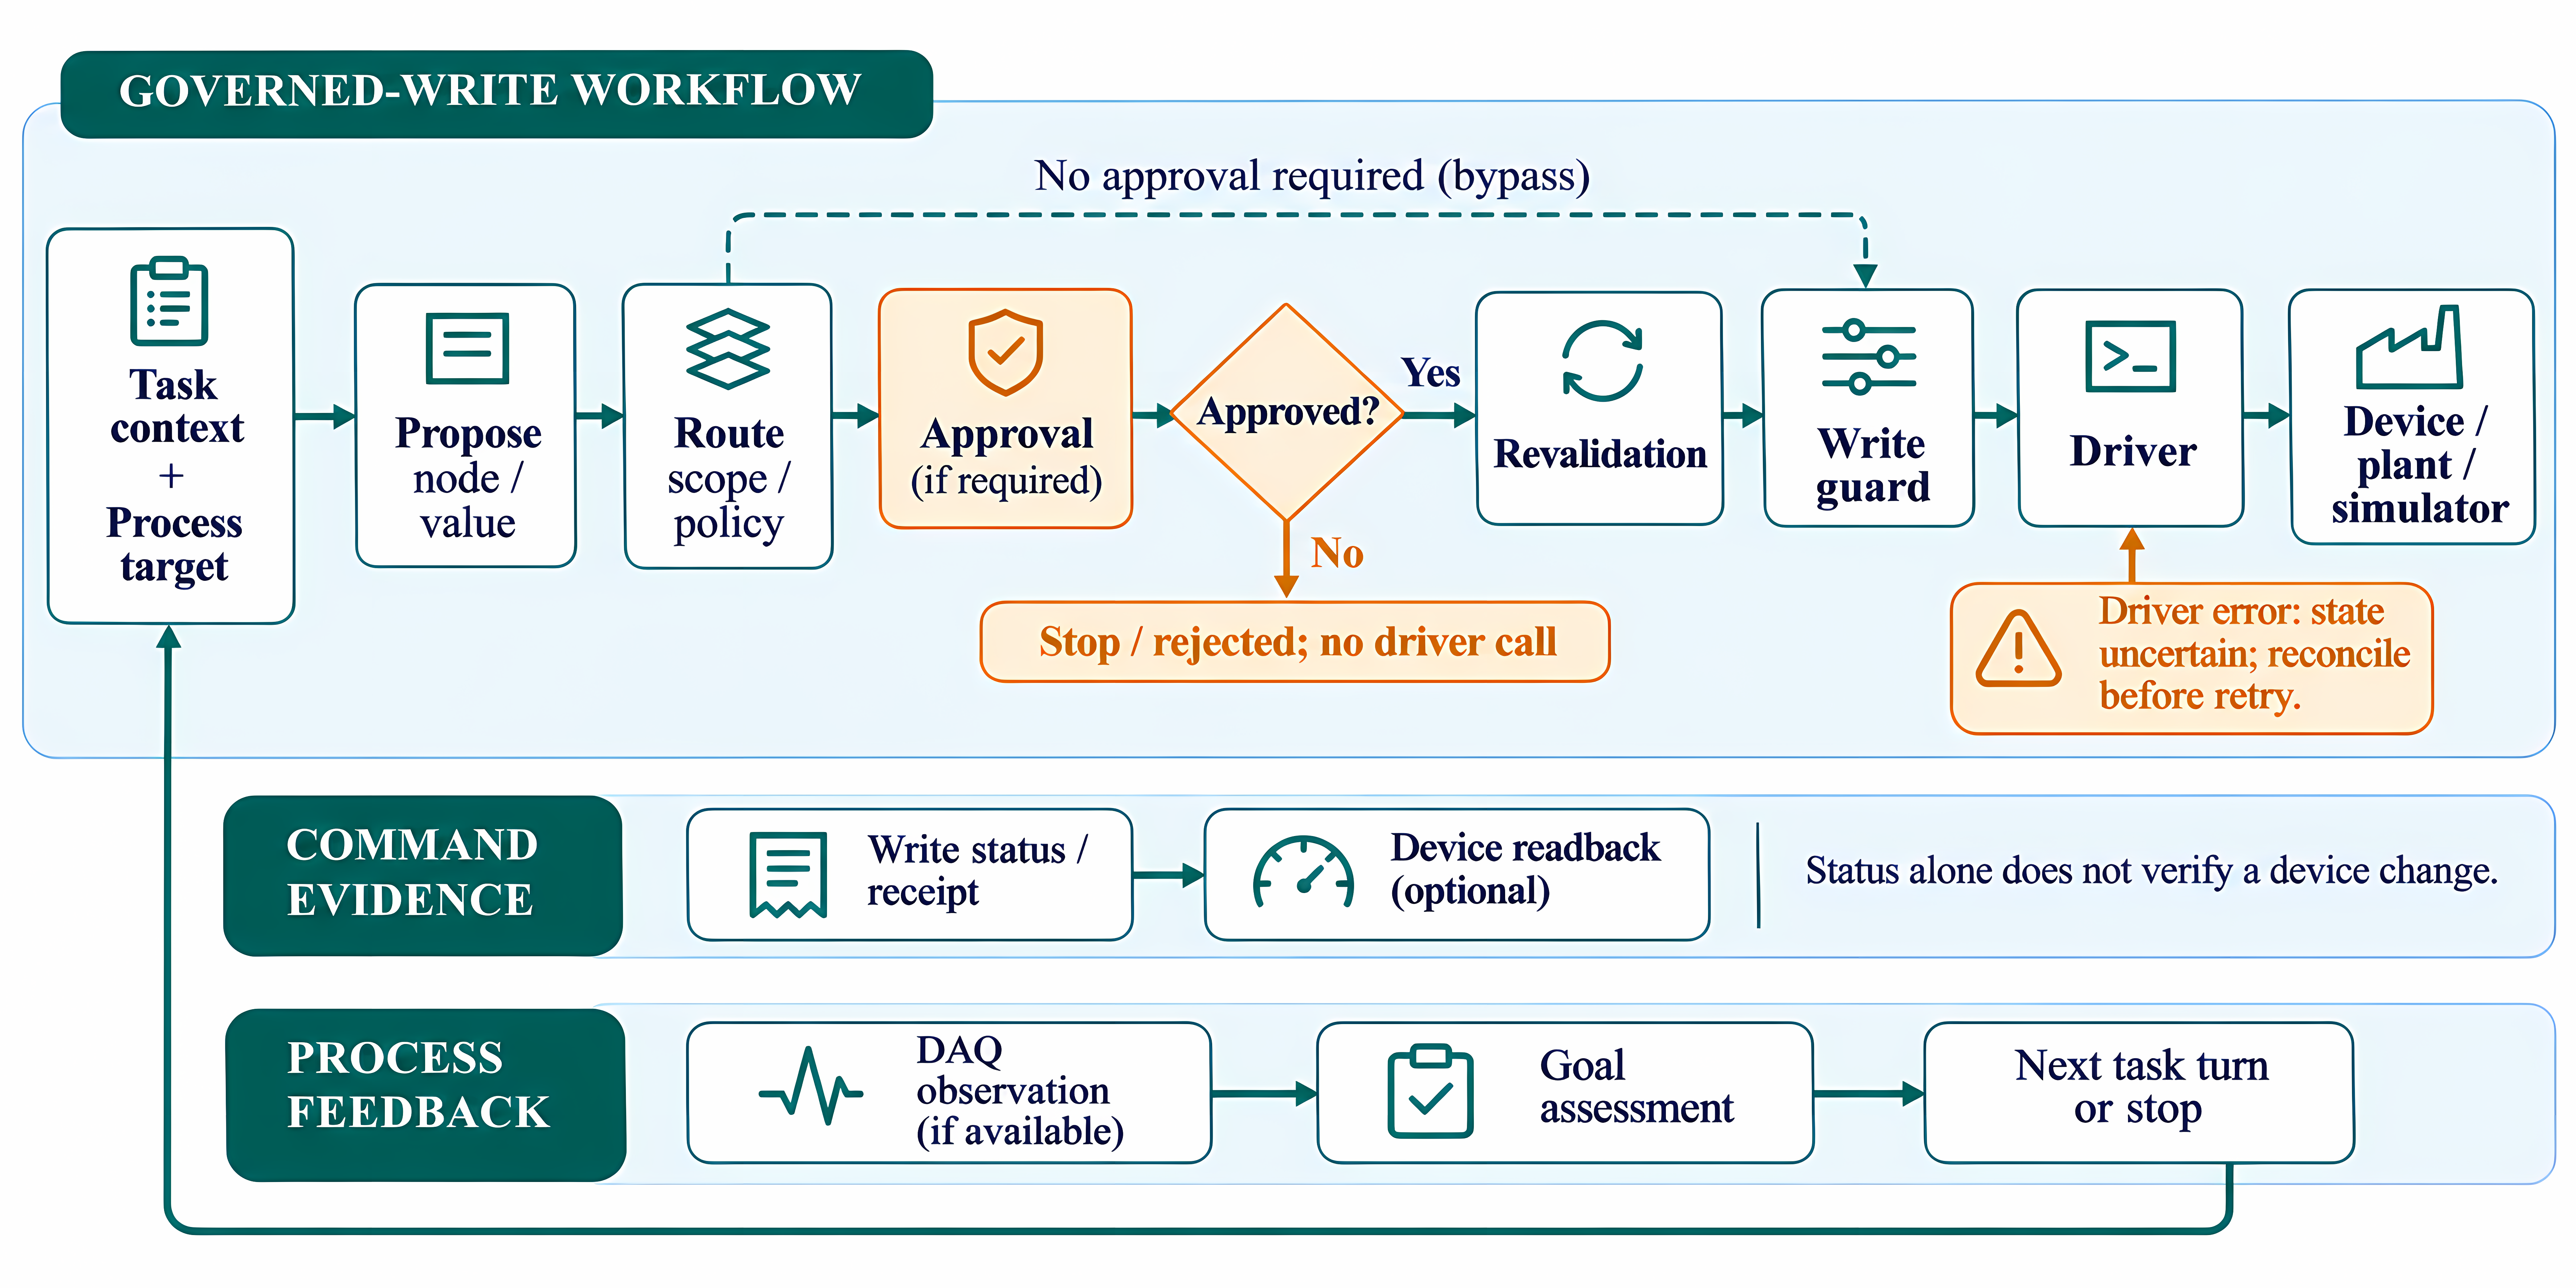
\includegraphics[width=\textwidth]{../figures/fig3.png}
\caption{Conceptual governed-write workflow. The task context supplies a process goal, and the Agent proposes a node/value that passes route-scope and policy checks. Requests requiring approval proceed through the decision and, if approved, revalidation; requests that do not require approval bypass those stages but still enter the write guard. Rejection stops before any driver call. A driver-stage error may leave device state uncertain and require reconciliation. The figure separates a write status/receipt and optional device readback from later DAQ feedback and goal assessment on a subsequent task turn. It describes the workflow, not an observed live-Agent success.}
\label{fig:agent-loop}
\end{figure*}

\section{Operation Governance and Evidence}
\label{sec:modules}
Section~\ref{sec:design} defines the shared dispatch contract. This section
focuses on the checks that follow it: scene-specific write admission,
conditional approval, and the records returned by each route.

\subsection{Scene-Specific Write Admission}
\label{sec:governed}
After shared dispatch checks pass, the selected handler applies the limits
configured for the scene and control node. Authorization and value admission
are separate checks. The target band describes a desired process outcome; it
does not define the admissible write interval. A candidate can satisfy every
write constraint while the measured process value remains outside the target
band.

For an online node write, the admissible value interval is
\begin{equation}
\mathcal{I}^{\mathrm{online}}_n(t)=
\mathcal{H}_n\cap\mathcal{L}^{\mathrm{base}}_n\cap\mathcal{L}^{\mathrm{prod}}_n(t)\cap\mathcal{L}^{\mathrm{rec}}_n(t),
\label{eq:admission}
\end{equation}
where $\mathcal{H}_n$ is the hard engineering range, and
$\mathcal{L}^{\mathrm{base}}_n$, $\mathcal{L}^{\mathrm{prod}}_n$, and
$\mathcal{L}^{\mathrm{rec}}_n$ are the baseline, active-product, and
active-recipe limits. These numerical bounds are distinct from the scope,
policy, grant, and binding predicates in Eq.~(\ref{eq:dispatch-contract}).
Missing optional limits impose no restriction. If the intersection is empty,
the request is rejected and the excluding layer is identified. Recipe dispatch checks a
replacement recipe against the hard, baseline, and product limits rather than
the previous recipe's window; trial overrides are also checked against the
applicable recipe window. Outside benchmark mode, step, interval, and
hold-window rules apply to agent- or manual-source writes. Recipe and rollback
writes follow their own paths. These application-level checks complement, but
do not replace, equipment interlocks.

\subsection{Approval, Execution, and Evidence}
\label{sec:mech}
Approval depends on the operation route. For a single-node
\texttt{optimization\_explore} request in manual mode, the handler sends the
node, requested value, current effective interval, and rationale to the
approval service. It waits for a decision before calling the governed write
operation; a decline or timeout returns without reaching the controller, and
no dispatch occurs while the request is pending. Once approved, the handler
rechecks the node binding and applicable channel grant. The shared controller
then evaluates the current engineering, parameter, product, and recipe limits.
Outside benchmark mode, agent- or manual-source writes also face step,
interval, and hold-window checks before dispatch to the configured driver.
Unlike the recipe path described below, this single-node path does not use a
recipe-operation context snapshot. Revalidation does not establish an atomic
snapshot spanning the external device write.

Recipe operations follow a separate approval path. For \texttt{recipe\_trial}
and \texttt{recipe\_apply}, approval is bound to the operation and active
line--product--recipe--run context. After approval, the handler rechecks
authority and context, then verifies the recipe definition and candidate scope
before dispatch. A changed context, revoked binding, or changed recipe
definition prevents the proposal from proceeding. Recipe-trial approvals
remain valid for 30 minutes by default; single-node approval waits expire
after 180\,s. Outside benchmark mode, agent- and manual-source writes require
at least 60\,s between setpoint changes; recipe trials also use a default
per-line cadence of 300\,s.

Fig.~\ref{fig:hitl} contrasts the bounds used for online node writes in
Eq.~(\ref{eq:admission}) with those used for a replacement recipe, and shows
the route-dependent approval and shared-dispatch paths.

\begin{figure*}[t]
\centering
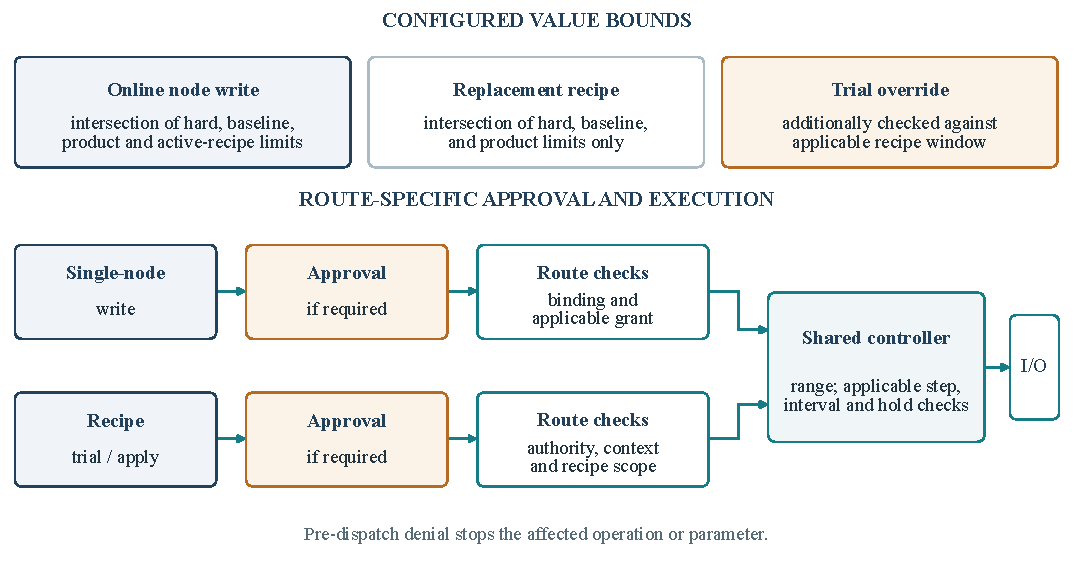
\includegraphics[width=\textwidth]{../figures/fig4.pdf}
\caption{Write admission and route-dependent approval. An online node write uses the intersection of hard, baseline, product, and active-recipe bounds; a replacement recipe is checked against hard, baseline, and product bounds, not the previous recipe window. Trial overrides are additionally checked against the applicable recipe window. After required approval, the routes recheck their applicable binding, grant, context, and recipe scope. The shared controller applies range checks; step, interval, and hold-window checks apply to agent or manual sources outside benchmark mode. A failed pre-dispatch check prevents the affected operation or parameter from reaching the driver.}
\label{fig:hitl}
\end{figure*}

A \texttt{recipe\_trial} illustrates this path. The handler checks the bound
recipe, active run, candidate parameters, and route timing. If approval is
required, it requests a decision and then revalidates authority and context
before submitting a bounded batch through the configured driver. It returns a
result for each parameter. Parameters are attempted individually, so a batch
can be partially applied; the per-parameter results and device state must be
reconciled before retrying. A trial does not save or apply a recipe version.
Callers can retrieve later DAQ observations separately before updating,
applying, or rolling back a recipe. The driver registry maps semantic controls
to configured protocol drivers, so operation arguments contain no
protocol-specific details.

Receipts record command outcomes; observations record subsequent process
behavior. Command results are graded as readback-verified,
transport-acknowledged, or unverified. A readback mismatch can trigger up to
three reads at 2\,s intervals, and recipe batches retain verification
outcomes for each parameter. A readback-verified result means that the
returned value matched the request. A transport acknowledgement alone does not
establish that the device applied the value, and an unverified result does not
establish a matching readback. DAQ stores later timestamped process
observations; recipe history, approvals, and task records remain with
their owning services. Identifiers and timestamps can link these records
when available, but a later observation alone does not prove that the command
caused the measured change. Section~\ref{sec:eval} evaluates selected parts
of this evidence chain under the stated test conditions.



\section{Experimental Evaluation}
\label{sec:eval}
The core experimental records cover already-running platform and simulator services; no Agent harness was active in the integrated runs. The full active-service snapshot was not captured, so these results describe the recorded paths rather than a frozen release. The architecture defines task-mediated and direct routes to shared dispatch, but the experiments do not establish end-to-end execution through a registered harness or equivalence between the entry paths.

Most blocks used benchmark mode, which relaxes normal timing and hold-window controls; separate production-mode guard checks are reported on their own. No cold-start deployment or physical-plant run was performed. The evaluation follows selected paths from configured mapping and write admission to process observations and exploratory Agent episodes. Because the blocks use different units—mapping requests, fixed stimuli, per-seed endpoints, a single simulated-twin execution, and Agent episodes—the counts are not pooled.

Table~\ref{tab:evidence-scope} connects each evaluation block to the question it can answer. A matching readback checks the actuator value returned by the simulator; it does not establish a process response. Conversely, an in-band process observation does not by itself establish which write caused it. The route and guard checks address pre-dispatch behavior, whereas the live-Agent episodes address whether a task reached a governed write. These distinctions determine the scope of the conclusions below.

\begin{table*}[!t]
\centering
\caption{Evaluation blocks, observational units, and limits of interpretation.}
\label{tab:evidence-scope}
\footnotesize
\setlength{\tabcolsep}{5pt}
\begin{tabularx}{\textwidth}{@{}>{\raggedright\arraybackslash}p{0.19\textwidth}>{\raggedright\arraybackslash}p{0.18\textwidth}>{\raggedright\arraybackslash}p{0.28\textwidth}X@{}}
\toprule
Block & Unit & Observation & Interpretation boundary \\
\midrule
Mapping probes & Configured request & Acceptance, rejection, and available simulated readback & Same configured limits supply inputs and checks; no physical actuation \\
Guard ablation & Fixed stimulus and technical repetition & Hypertext Transfer Protocol (HTTP) response status & One scene; benchmark mode; no readback-mismatch stimulus \\
E6 paired comparison & Scene--seed pair & Trapezoidal IAE over a fixed horizon & 11 post-pilot attempts; 9 valid pairs, 2 invalid sampling records; exploratory scripted policy versus no-write \\
Injection-twin pilot & One scripted execution & Write receipt, readback, and later process observation & No replication; incomplete raw series and runtime provenance \\
E7 Agent pilot & Episode & Task status, process value, and recorder-reported writes & Three episodes; all canceled and below band; no archived server journal \\
\bottomrule
\end{tabularx}
\end{table*}

\subsection{Configured Mapping and Integration Checks}
\label{sec:eval-mapping}
Two integrated executions each passed 77 assertions across 17 phases. These assertions provide repeated checks of the configured service path; they are not independent trials.

The two executions used seed 42, started with the platform and simulator already running, and did not activate an Agent harness. A separate preset check within the integrated film-line path configured five endpoint types and rejected nine selected negative probes. It reused the same runtime, so it is not a cold-start deployment or an independent replication of the mapping matrix.

The scene--protocol probes covered 55 writable nodes across four simulated scenes and five configured protocol variants. The variants included Transmission Control Protocol (TCP), Modbus remote terminal unit (RTU) mode, OPC UA, MQTT, and HTTP. Each node received three interior-value requests, one upper-boundary request, and four structural-range requests. All 220 admissible requests were accepted; 219 collected structural-range requests were rejected; and all 216 available readbacks matched. These probes check the consistency of configured mappings: the tested values and guards use the same configured limits. Simulator readback echoes the configured value and does not verify physical actuation. One structural request was not collected, HTTP nodes do not expose readback, and the full scene--protocol matrix remains incomplete. The excluded cast-film run and other deviations are documented in Supplementary File~S7.

\begin{table*}[!t]
\centering
\caption{Scene--protocol probes. Admissible, structural, and readback columns give accepted, rejected, and matching counts from the frozen batch; window counts are from a separate follow-up batch. Readback counts include accepted requests for which the simulator exposes an actuator value.}
\label{tab:scene-probe-results}
\footnotesize
\setlength{\tabcolsep}{3pt}
\begin{tabularx}{\textwidth}{@{}>{\raggedright\arraybackslash}p{1.55cm}r X r r r r@{}}
\toprule
Scene & Nodes & Protocols represented & Admissible & Structural & Readback & Window$^{\dagger}$ \\
\midrule
Injection & 11 & TCP 5; RTU 2; OPC UA 3; MQTT 1 & 44/44 & 44/44 & 44/44 & 22/22 \\
Wastewater & 7 & TCP 1; RTU 3; OPC UA 2; MQTT 1 & 28/28 & 28/28 & 28/28 & 14/14 \\
Annealing & 7 & TCP 3; RTU 2; OPC UA 1; MQTT 1 & 28/28 & 28/28 & 28/28 & 14/14 \\
Biaxial line & 30 & TCP 20; RTU 1; OPC UA 8; HTTP 1 & 120/120 & 119/119 & 116/116 & 60/60 \\
\bottomrule
\end{tabularx}\\
{\footnotesize $^{\dagger}$ Follow-up batch: recipe-window violations rejected / tested; counts are not pooled with the frozen batch.}
\end{table*}

\subsection{Write-Guard and Route Checks}
\label{sec:eval-ablation}
The ablation used one scene, direct API calls, a mock driver, and three deterministic repetitions per guard setting in benchmark mode. Each repetition submitted four structural-range violations and two process-window violations, as well as three legal and three boundary requests. The timed writes used for latency summaries were excluded from these counts. With all guards enabled, all six targeted process-window violations returned HTTP 400. With the process-window check removed, all six returned HTTP 200; structural violations continued to be rejected. The four structural violations were rejected in every repetition and setting; the nine legal requests per setting were accepted and the nine boundary expectations were met. These deterministic fixture counts are not independent trials or a safety rate. The archive lacks response bodies and per-request driver-call logs, so an HTTP 200 response alone does not establish driver invocation; the experiment included no readback-mismatch stimulus.

Separate scripted probes reached the expected approval and authorization branches. In the manual approval fixture, the approved request changed the simulated value from 202 to 204.8, while the rejected request left it at 216. The corresponding automatic calls did not form clean matched pairs because their labels and values did not align with those of the manual arms. No operator made the approval decisions. The probes show route handling in the tested fixture, not the effect of human approval or a general safety rate.

In a November 5 follow-up, a separate four-scene probe batch returned \texttt{RECIPE\_LIMIT\_EXCEEDED} for all 110 tested requests outside their configured recipe windows but within structural limits. The deterministic inputs and checks derive from the same configuration, so the count assesses the selected cases rather than a population failure rate. In a separate simulated injection-node fault injection, a 230-unit command produced a 251-unit readback against a 0.7-unit tolerance and was reported as \texttt{unverified}; one baseline and one recovery returned \texttt{readback-verified}. This tests one injected mismatch, not physical-device behavior. The later batch is not pooled with the frozen core results; its records and provenance limits are in Supplementary File~S7.

In a separate production-mode check, one legal baseline was accepted, and one case each was rejected for interval, step, node-range, recipe-window, and hold-window constraints. A three-case authorization probe rejected an unbound request and a cross-node request while accepting a bound write. These individual branch checks complement the benchmark-mode ablation but do not measure coverage across configurations. Full call records are listed in Supplementary File~S7.

\subsection{Fixed-Horizon Process Comparison}
\label{sec:eval-optimization}
The E6 comparison evaluated the paper's deterministic \texttt{recipe\_trial} policy (C1) against a no-write control (C0) in three simulated scenes: injection, wastewater, and annealing. The plan fixed four seeds per scene, independent fresh resets for each arm, setpoint verification, and a pre-registered initial-process-value window. Arm order was randomized within each block. The horizons were 180~s for injection and 240~s for the other scenes, with 1-s sampling. The primary outcome was trapezoidal integral absolute error (IAE); for each valid pair, $\Delta\mathrm{IAE}=\mathrm{IAE}_{C0}-\mathrm{IAE}_{C1}$, so a positive value indicates lower IAE under the scripted policy. The injection seed-43 block was designated as a pilot and is excluded from the comparison. Blocks 2--12 therefore provide 11 post-pilot attempts. A pair was valid only when both arms met the reset, initial-state, and trajectory-coverage criteria; pairs with a sampling gap greater than 5~s were retained as invalid and not replaced.

Nine of the 11 post-pilot attempts were valid, and each had a positive $\Delta\mathrm{IAE}$. The per-scene median differences were 165.165~g\,s for injection (3/3 valid pairs), 615.605~mg/L\,s for wastewater (3/4), and 8000.45~HV\,s for annealing (3/4). The valid-pair ranges were 162.535--195.169, 611.670--630.980, and 7930.200--8084.150 in the corresponding native units multiplied by seconds. The two invalid pairs were wastewater seed~45 (a 9-s gap in C0) and annealing seed~46 (a 6-s gap in C0). The separate injection pilot had $\Delta\mathrm{IAE}=163.240$~g\,s and is reported only in S7. Fig.~\ref{fig:latest-evaluation}(a) displays the nine valid paired differences and their per-scene medians. This small exploratory comparison tests one scripted policy against no-write in simulation; it is not a powered estimate, a comparison with PID, or evidence of LLM policy performance. Seeds index simulator initializations, not independent production lines.

\begin{figure*}[!t]
\centering
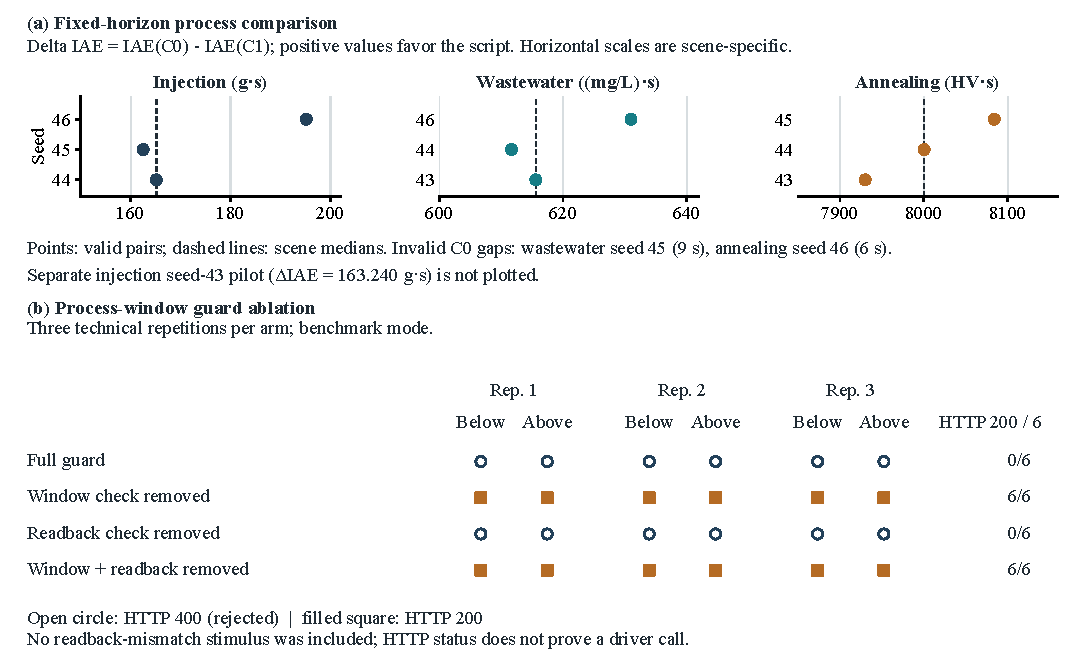
\includegraphics[width=\textwidth]{../figures/fig5.pdf}
\caption{Matched-horizon process comparison and guard-ablation responses. (a) Each point is a valid E6 scene--seed difference $\Delta\mathrm{IAE}=\mathrm{IAE}_{C0}-\mathrm{IAE}_{C1}$; vertical dashed lines show per-scene medians. Positive values indicate lower IAE under the scripted policy. Wastewater seed~45 and annealing seed~46 are excluded because of C0 sampling gaps; the separate seed-43 pilot is not plotted. The axes use scene-specific native units multiplied by seconds. (b) Each marker is a below- or above-window request in one of three technical repetitions. Open circles denote HTTP 400 and filled squares HTTP 200; the fractions give HTTP 200 counts. Structural checks remained enabled.}
\label{fig:latest-evaluation}
\end{figure*}

\subsection{Follow-Up Injection-Twin Pilot}
\label{sec:eval-followup-pilot}
An acceptance script later ran one end-to-end experiment on an isolated platform connected to a PLC-based simulated twin; the manifest records \texttt{realPlant=false}. At 50~bar, the structured record gives a baseline product weight of 31.503~g, below the 32.00--32.30~g band. Its accompanying report instead gives 31.508~g; the discrepancy remains unresolved. A three-level plan tested 50, 55, and 60~bar. The saved ledger labels its contrasts \texttt{no\_resolvable\_effect}, \texttt{underpowered}, and \texttt{identifiable\_effect}; it stores effect, minimum detectable effect (MDE), and verdict fields. The archive lacks the sample series and the rule used to calculate MDE and assign the labels. The final 55-to-60~bar contrast stores an effect of 0.2517~g over a 5-bar step; 0.05035~g/bar is that single-run ratio, not a replicated or independently verified process model.

The subsequent governed write changed the setpoint from 60 to 63.7~bar, and the device readback matched. After 60~s, the mean of the three latest 15-s process samples was 32.224~g, within the band. The reported 15/15 reflects assertions in this single execution, not trials. The record does not identify the platform source, simulator configuration, or runner source. This pilot demonstrates one scripted simulator path only; its records and provenance limits are in Supplementary File~S7.

\subsection{LLM-Driven Simulator Pilot}
\label{sec:eval-agent}
The latest E7 pilot comprised three injection episodes on the simulator. Each ended with task state \texttt{CANCELED} and a recorded process value below the 32.15--32.85~g target band: 31.70, 31.87, and 31.99~g. The episode recorder logged two writes in two rounds for each run; one episode carried a false guard-status flag. Episodes ended after 372--380~s, although the configured budget was 20~min. The saved episode package contains no server-side journal export, so these write counts are recorder-reported and cannot be independently reconciled with the parameter ledger. The runs are a pilot, not a success-rate estimate, and are not paired with E6. Earlier exploratory batches are retained separately in S7 and are not pooled with these episodes. No result here establishes task completion, physical-device execution, or general Agent reliability.

\section{Discussion}
\label{sec:discussion}
The tests show how the configured runtime handled the cases exercised here. Mapping probes exercised configured signal bindings, and the process-window ablation showed that the tested mock-driver route rejected the six selected out-of-window requests when the interlock was enabled. In the E6 comparison, all nine valid pairs had lower IAE under the deterministic recipe policy than under no-write. This is an exploratory result from a small simulated sample, not a general control-effect estimate. The earlier 15/15 versus 0/15 endpoint counts used different horizons and endpoint rules and remain historical descriptive evidence in Supplementary File~S7.

The three E7 episodes ended canceled and below the target band. Their local recorder reported two writes per episode, but the archive lacks a server-side journal for independent reconciliation. The task-mediated and direct routes share dispatch in the design, but route equivalence and cross-harness robustness were not tested. The single twin run also lacks raw samples and a frozen runtime snapshot. More broadly, the guard ablation had no readback-mismatch stimulus, approvals were scripted, and no PID baseline, operator study, or physical-plant evaluation was performed. A larger preregistered process comparison with complete source and event records is needed to estimate control effects; Agent execution and approval quality require separate task-level and human-operator studies. Simulator and mock-driver checks complement, but do not replace, PLC, safety instrumented system (SIS), and equipment protections.

\section{Conclusion}
\label{sec:conclusion}
The runtime binds production context and direction-specific mappings to shared dispatch, then applies route-specific checks before a write reaches a registered driver. It also keeps command outcomes, optional readbacks, and later process observations as separate records. In the tested simulator configurations, mapping probes exercised selected bindings, the guard ablation rejected the targeted window violations when the interlock was enabled, and nine valid E6 pairs showed lower IAE under the deterministic scripted policy than under no-write. The E6 result is exploratory; the three E7 episodes were canceled and did not reach the target band. These results do not establish general control efficacy, reliable autonomous task execution, operator decision quality, or physical-plant safety. Larger controlled process comparisons and complete Agent and operator studies remain open.


\section*{Declarations}
Author contributions are declared in the submission system; no competing
interests are declared.

\section*{Data Availability}
Supplementary File~S7 contains run manifests, raw CSVs, per-seed outcomes, guard ablations, and scenario-pilot records. Separate archives preserve the preregistered E6 plan and per-arm trajectories, the E6 pilot, and the three E7 episode records and traces. The E7 archive does not contain the reported server-side journal export. No physical-plant data were collected.

\bibliographystyle{IEEEtran}
% Balance the reference columns on the final page.
% Column balancing is deferred to the final production proof.
\bibliography{resources/refs}

\end{document}

